\section{实验步骤}
\subsection{实验准备}
在修改源代码前,将先前实验内容在本地提交,并如图\ref{push}所示,上传至GitLab中保管。然后如图\ref{dev}所示,创建并切换至分支 \texttt{dev}。

\begin{figure}[!htbp]
    \centering
    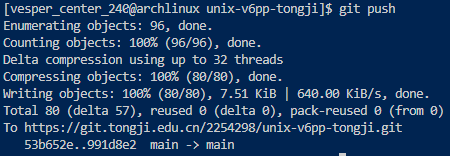
\includegraphics[scale=1]{images/push.png}
    \caption{将代码上传至GitLab中}\label{push}
\end{figure}

\begin{figure}[!htbp]
    \centering
    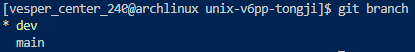
\includegraphics[scale=1]{images/dev.png}
    \caption{切换至分支 \texttt{dev}}\label{dev}
\end{figure}


\subsection{修改页表构建过程}
如图\ref{breakpoint}所示,修改源代码之前,执行 \texttt{make qemu}, 命中\texttt{EstablishUserPageTable}函数体内的断点时,
日志显示 \texttt{textVirtualAddress}为4M+4K, \texttt{textSize}为16K, \texttt{dataVirtualAddress}为4M+20K, \texttt{dataSize}为24K, \texttt{stackSize}为4K。

\begin{Verbatim}[frame=single,fontsize=\small,commandchars=\\\{\}]
Breakpoint 2, MemoryDescriptor::EstablishUserPageTable (this=0xc03ff014, textVirtualAddress=4198400, textSize=16384, dataVirtualAddress=4214784, dataSize=24576, stackSize=4096) at /home/vesper\_center\_240/unix-v6pp-tongji/src/proc/MemoryDescriptor.cpp:100
\end{Verbatim}
\captionof{figure}{命中\texttt{EstablishUserPageTable}函数体内的断点}\label{breakpoint}

  由于我使用 \texttt{git}进行版本控制,所以直接在源代码中修改。如果需要,可以使用 \texttt{git stash}和 \texttt{git stash pop}切换修改前后的源代码版本。

  在本阶段的修改中,我在达成修改目的的前提下,尽可能地减少修改的幅度,并保持修改前后的代码风格一致。因此,我将\texttt{MapEntry}进行修改,用于直接计算得到页表。
为了保持参数表一致,我将 \texttt{m\_UserPageTableArray}成员改为 \texttt{UserPageTableArray},以便能够在 \texttt{MapEntry}函数体内进行读取。
其余修改则是根据编译器的报错进行的,主要内容是把 \texttt{MemoryDescriptor}类的成员函数中对\texttt{m\_UserPageTableArray}成员的使用部分删去。

  图\ref{member}-\ref{MapToPageTable}为本阶段所作修改。修改过后,可以成功编译并正常运行。代码\ref{lst:h},\ref{lst:cpp}为本实验完成时的完整代码。修改的核心思想在于
修改原先用于构建相对虚实地址映射表的辅助函数 \texttt{MapEntry}以用于直接构建用户态页表,在 \texttt{MapToPageTable}中只需像 \texttt{EstablishUserPageTable}中构建虚实地址映射表一样,将各段的虚拟地址、段大小、起始物理页框传入即可。

\begin{figure}[!htbp]
    \centering
    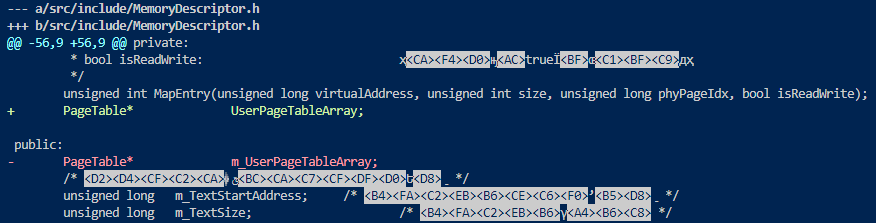
\includegraphics[width=\textwidth]{images/member.png}
    \caption{修改 \texttt{MemoryDescriptor}成员}\label{member}
\end{figure}

  如图\ref{SetupProcessZero}所示, \texttt{SetupProcessZero}函数体内对于 \texttt{m\_UserPageTableArray}的赋值直接删去即可。

\begin{figure}[!htbp]
    \centering
    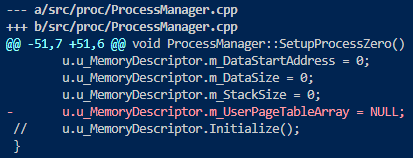
\includegraphics[scale=1]{images/SetupProcessZero.png}
    \caption{对 \texttt{SetupProcessZero}的修改}\label{SetupProcessZero}
\end{figure}


  如图\ref{NewProc}所示,\texttt{NewProc}中对\texttt{m\_UserPageTableArray}的使用是由于在父进程拷贝自身图像给子进程时,需要在自身和子进程的相对虚实映射表之间切换。
由于现在彻底移除了对于相对虚实地址映射表的使用,所以相关代码直接移除即可。

\begin{figure}[!htbp]
    \centering
    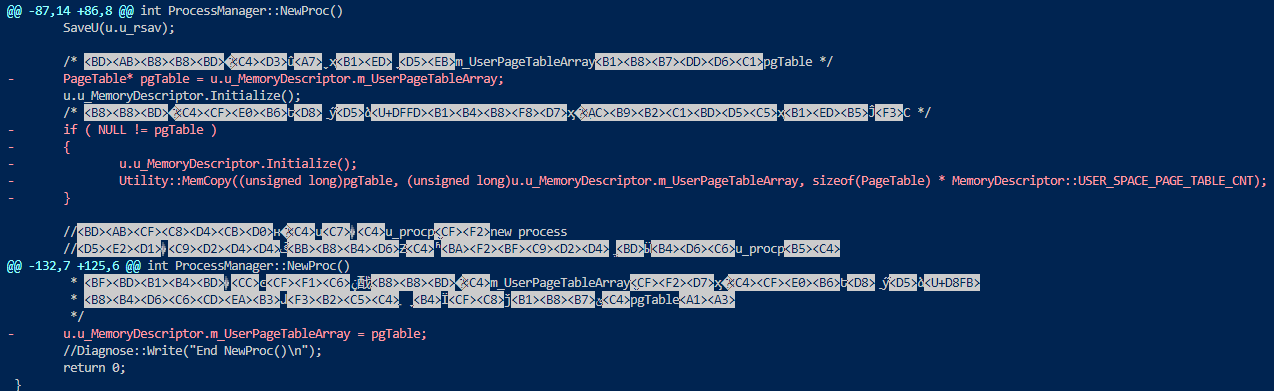
\includegraphics[width=\textwidth]{images/NewProc.png}
    \caption{对 \texttt{NewProc}的修改}\label{NewProc}
\end{figure}

  如图\ref{initRel}所示,为了能够在 \texttt{MapEntry}函数体内进行读取\texttt{UserPageTableArray},我在\texttt{Initialize}中为其赋值(后续会将\texttt{Initialize}彻底删除) 。
\texttt{Release}的作用时用于释放相对虚实地址映射表所占用的内存空间,由于现在彻底移除了对于相对虚实地址映射表的使用,所以相关代码直接移除即可。

\begin{figure}[!htbp]
    \centering
    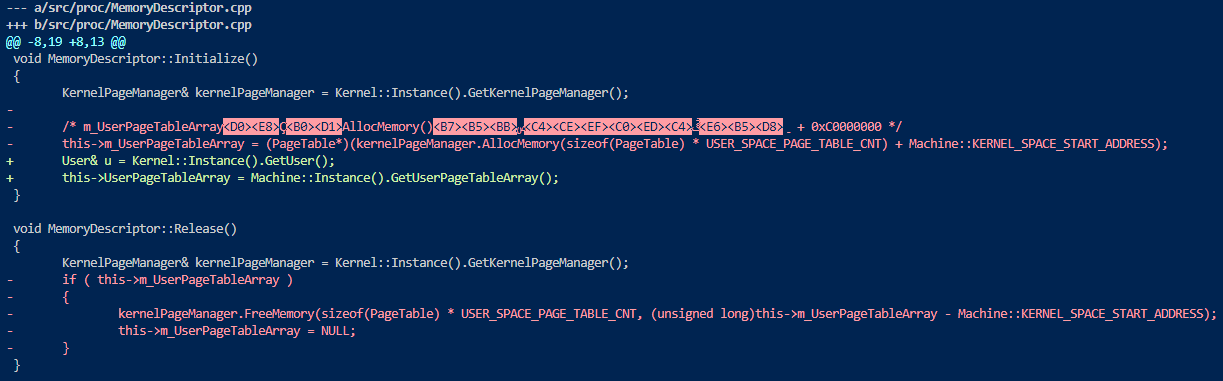
\includegraphics[width=\textwidth]{images/Initialize_Release.png}
    \caption{对 \texttt{Initialize}和 \texttt{Release}的修改}\label{initRel}
\end{figure}

  如图\ref{MapEntry}所示,这一修改使得\texttt{MapEntry}直接构建用户态页表,而非相对虚实地址映射表。

\begin{figure}[!htbp]
    \centering
    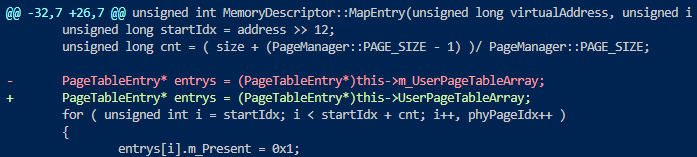
\includegraphics[width=\textwidth]{images/MapEntry.png}
    \caption{对 \texttt{MapEntry}的修改}\label{MapEntry}
\end{figure}

  如图\ref{delete}所示,
由于现在彻底移除了对于相对虚实地址映射表的使用,所以可以直接移除用于获取其的接口。

\begin{figure}[!htbp]
    \centering
    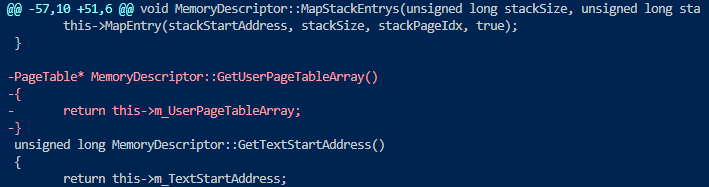
\includegraphics[width=\textwidth]{images/delete.png}
    \caption{删除 \texttt{GetUserPageTableArray}}\label{delete}
\end{figure}

  如图\ref{EstablishUserPageTable}所示,
由于现在彻底移除了对于相对虚实地址映射表的使用,初始化它的相关代码可以直接移除。

\begin{figure}[!htbp]
    \centering
    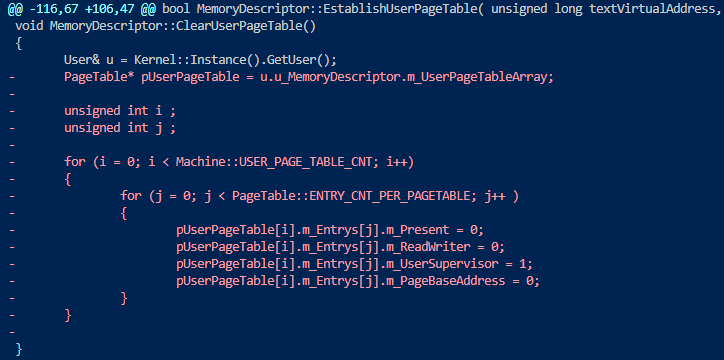
\includegraphics[width=\textwidth]{images/EstablishUserPageTable.png}
    \caption{对  \texttt{EstablishUserPageTable}的修改}\label{EstablishUserPageTable}
\end{figure}

  如图\ref{MapToPageTable}所示,保留循环中置存在位为0的部分,然后在循环后仿照 \texttt{EstablishUserPageTable}直接创建用户态页表,其中各段的虚拟起始地址、大小、物理起始地址通过\texttt{User}结构和\texttt{MemoryDescriptor}成员值获得。

\begin{figure}[!htbp]
    \centering
    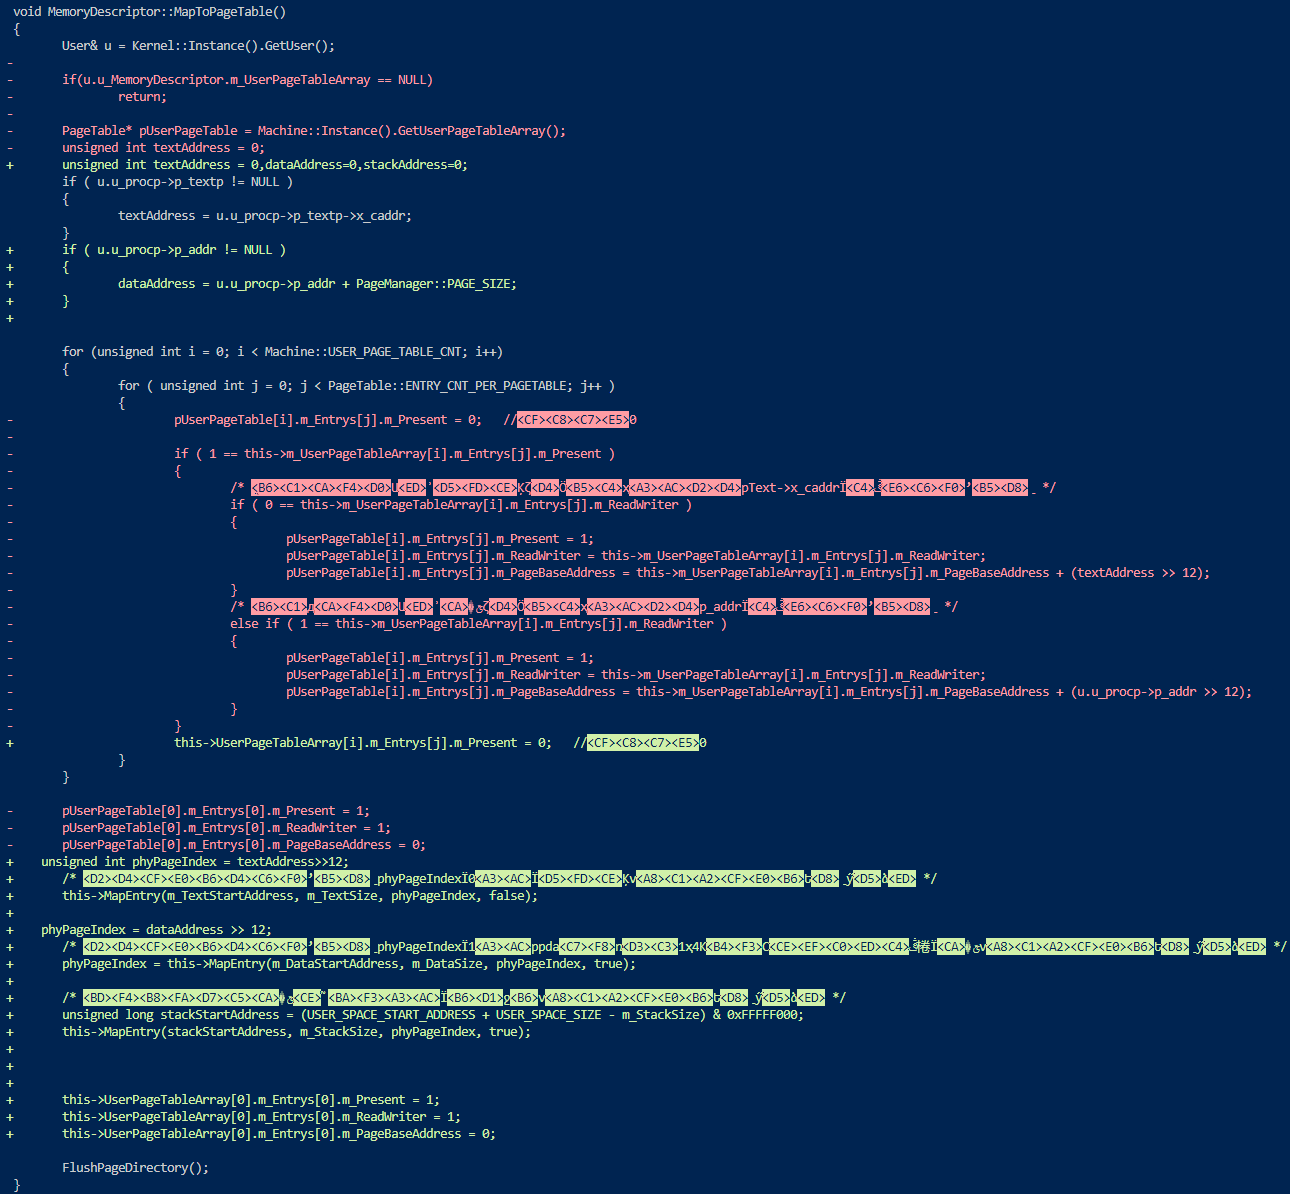
\includegraphics[width=\textwidth]{images/MapToPageTable.png}
    \caption{对 \texttt{MapToPageTable}的修改}\label{MapToPageTable}
\end{figure}



\clearpage
\subsection{删除 \texttt{MemoryDescriptor}类中其他与相对虚实地址映射表有关的函数}

  如图\ref{h}-\ref{deleteEstablishUserPageTable}所示,在本阶段中,所作主要修改为删除 \texttt{MemoryDescriptor}中于相对虚实地址映射有关的函数以及对于它们的调用。

  如图\ref{deleteInitRel},\ref{changeMapToPageTable}所示,由于删除了 \texttt{Release}函数,所以对于 \texttt{UserPageTableArray}的赋值移动至 \texttt{MapToPageTable}函数体内。
如图\ref{deleteRelease},\ref{deleteInitialize}所示,在\texttt{Exit},\texttt{NewProc}中,分别调用了\texttt{Release}和\texttt{Initialize},
由于现在彻底移除了对于相对虚实地址映射表的使用,所以可以直接移除这两处调用。


\begin{figure}[!htbp]
    \centering
    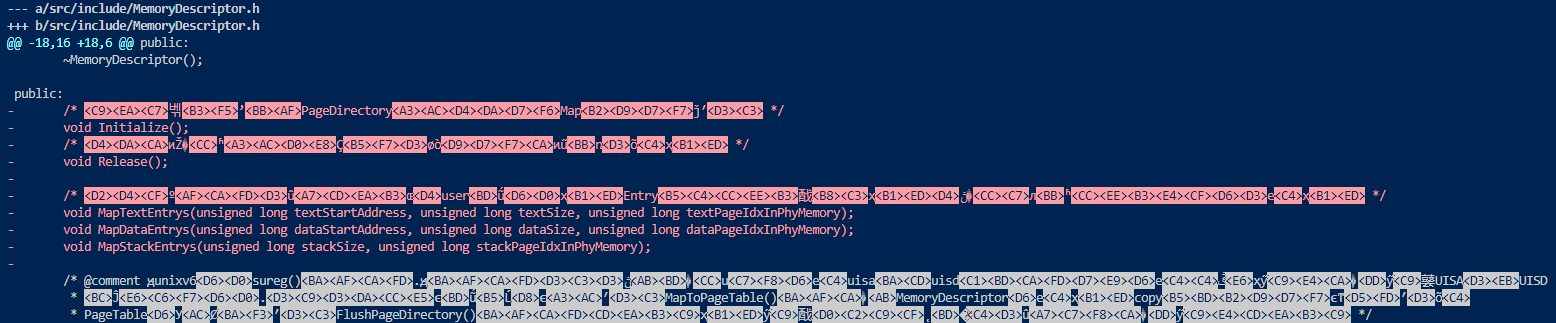
\includegraphics[width=\textwidth]{images/h.png}
    \caption{对 \texttt{MemoryDescriptor.h}的修改}\label{h}
\end{figure}

\begin{figure}[!htbp]
    \centering
    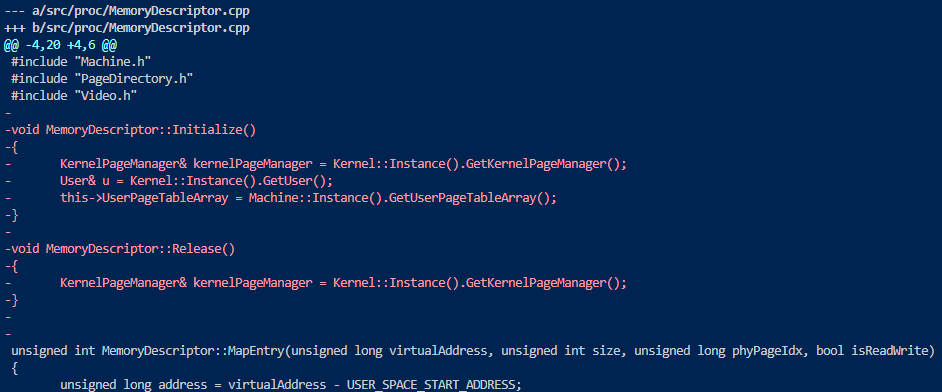
\includegraphics[width=\textwidth]{images/deleteInitRel.png}
    \caption{删除 \texttt{Initialize}和 \texttt{Release}}\label{deleteInitRel}
\end{figure}

\begin{figure}[!htbp]
    \centering
    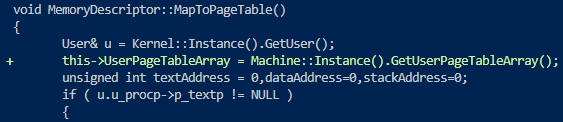
\includegraphics[scale=1]{images/changeMapToPageTable.png}
    \caption{修改 \texttt{MapToPageTable}}\label{changeMapToPageTable}
\end{figure}

\begin{figure}[!htbp]
    \centering
    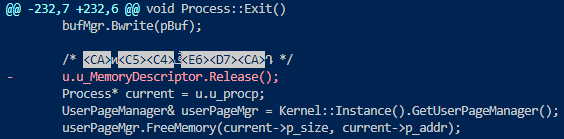
\includegraphics[scale=1]{images/deleteRelease.png}
    \caption{删除对 \texttt{Release}的调用}\label{deleteRelease}
\end{figure}

\begin{figure}[!htbp]
    \centering
    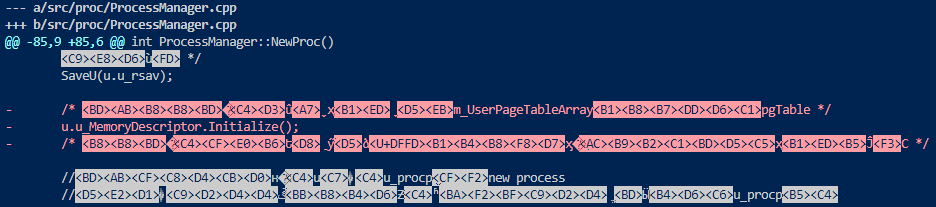
\includegraphics[width=\textwidth]{images/deleteInitialize.png}
    \caption{删除对 \texttt{Initialize}的调用}\label{deleteInitialize}
\end{figure}

  如图\ref{deleteEntry}所示,直接删去\texttt{MapTextEntrys}, \texttt{MapDataEntrys}和 \texttt{MapStackEntry}。它们实际上是针对
代码段,数据段和堆栈段进行封装的\texttt{MapEntry},但是在源代码中并没有调用。

\begin{figure}[!htbp]
    \centering
    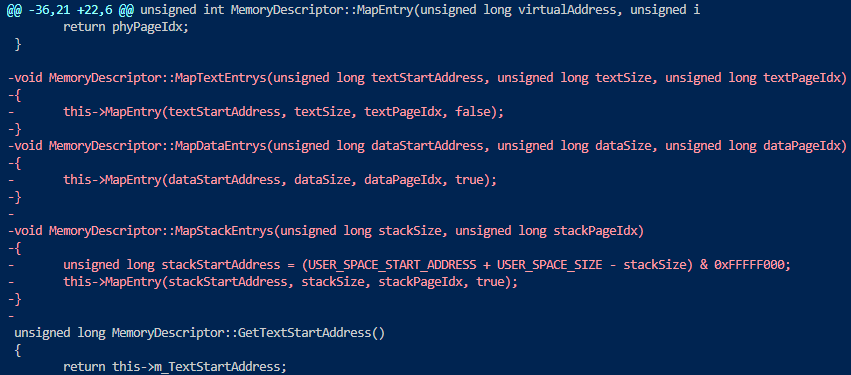
\includegraphics[width=\textwidth]{images/deleteEntry.png}
    \caption{删除 \texttt{MapTextEntrys}, \texttt{MapDataEntrys}和 \texttt{MapStackEntry}}\label{deleteEntry}
\end{figure}

如图\ref{deleteClearUserPageTable},
由于现在彻底移除了对于相对虚实地址映射表的使用,所以可以直接移除该用于清除相对虚实地址映射表的函数。

\begin{figure}[!htbp]
    \centering
    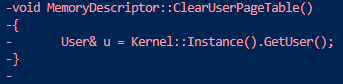
\includegraphics[scale=1]{images/deleteClearUserPageTable.png}
    \caption{删除 \texttt{ClearUserPageTable}}\label{deleteClearUserPageTable}
\end{figure}

  如图\ref{deleteEstablishUserPageTable}所示,遗留下来的初始化相对虚实地址映射表的代码部分被删除,在修改完\texttt{MapEntry}后,这一部分实际上直接作用于用户态页表,其作用部分会被后来调用的\texttt{MapToPageTable}所覆盖。
由于 \texttt{EstablishUserPageTable}中还有检测是否超出地址空间限制的部分,所以暂时不整体删除。
\texttt{MapEntry}由于已经修改为用于重构用户态页表的辅助函数,所以也不删去。

\begin{figure}[!htbp]
    \centering
    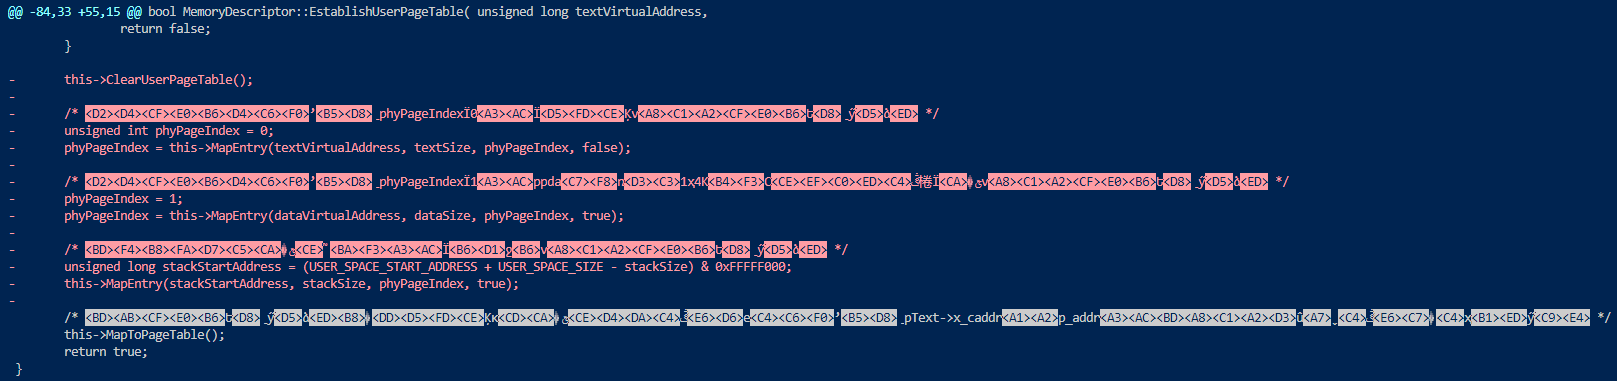
\includegraphics[width=\textwidth]{images/deleteEstablishUserPageTable.png}
    \caption{删除 \texttt{EstablishUserPageTable}中相关部分}\label{deleteEstablishUserPageTable}
\end{figure}


  接着,如图\ref{remain}-\ref{Exec}所示,我进一步将 \texttt{EstablishUserPageTable}完全删去,并其他文件中对其的调用。

  \texttt{EstablishUserPageTable}分别被 \texttt{SStack}, \texttt{SBreak}和 \texttt{Exec}调用。
\texttt{SStack}用于堆栈溢出时,自动扩展堆栈。在调用 \texttt{EstablishUserPageTable}之前,便以通过\verb|md.m_StackSize += charge|更新过堆栈大小,因此修改后的条件判断语句中,
各段的大小和起始地址可以直接从\verb|md|中获取;
\texttt{SBreak}用于扩展数据段,新的数据段大小为\verb|newSize|,因此修改过后的条件判断语句中,应用\verb|newSize|代替\verb|md.DataSize|;
\texttt{Exec}用于系统调用,进程图像切换,修改后的条件判断语句中,使用修改前参数表中的各局部变量即可。

  修改完成后,编译成功,运行正确。

\begin{figure}[!htbp]
    \centering
    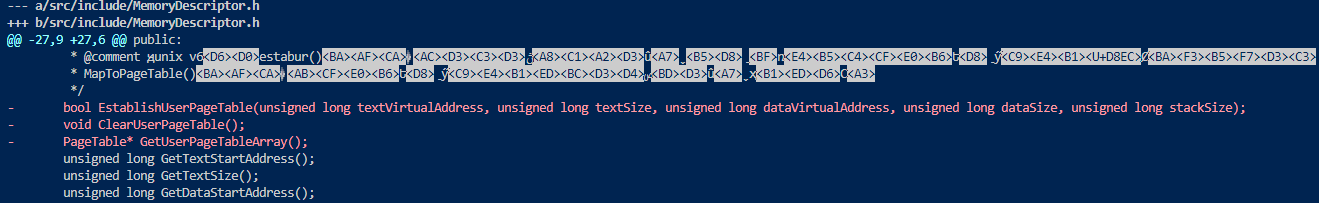
\includegraphics[width=\textwidth]{images/remain.png}
    \caption{删除 \texttt{MemoryDescriptor.h}中的遗留部分}\label{remain}
\end{figure}

\begin{figure}[!htbp]
    \centering
    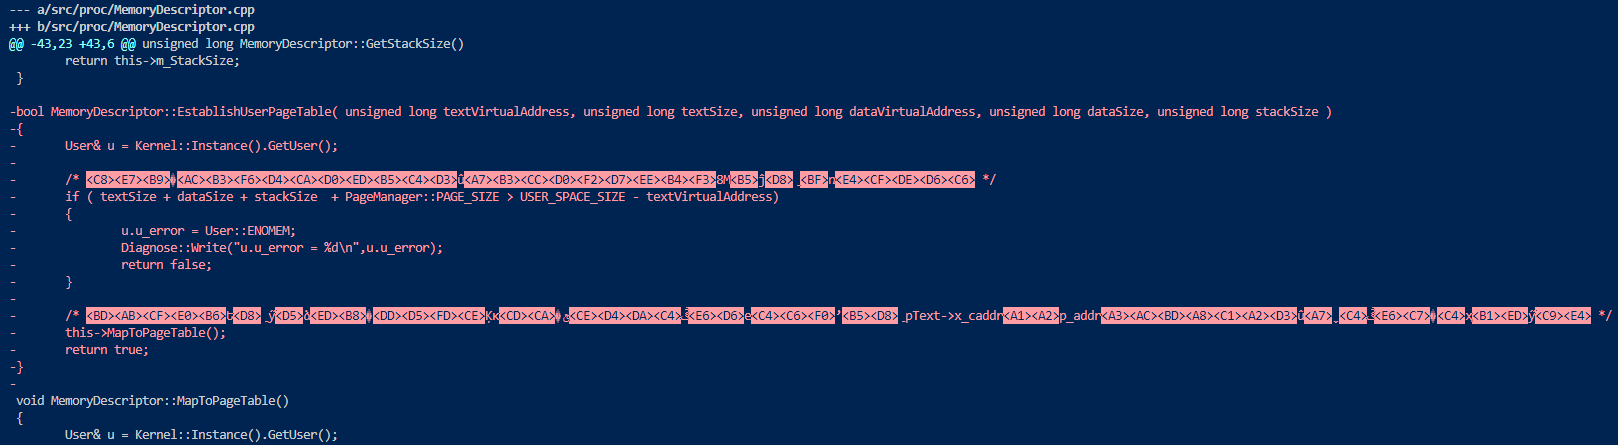
\includegraphics[width=\textwidth]{images/deleteAll.png}
    \caption{彻底删除 \texttt{EstablishUserPageTable}}\label{deleteAll}
\end{figure}

\begin{figure}[!htbp]
    \centering
    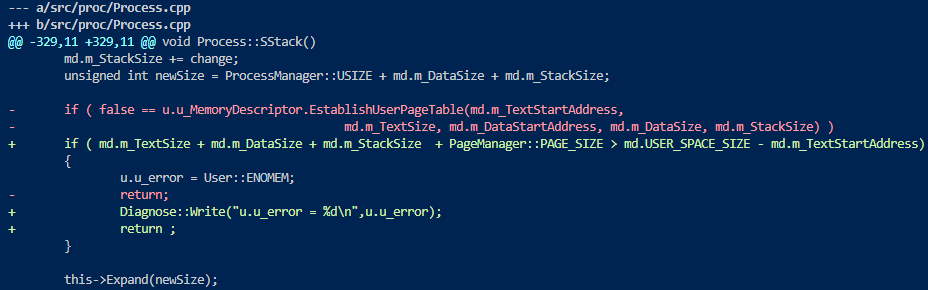
\includegraphics[width=\textwidth]{images/SStack.png}
    \caption{调整 \texttt{SStack}对 \texttt{EstablishUserPageTable}的调用}\label{SStack}
\end{figure}

\begin{figure}[!htbp]
    \centering
    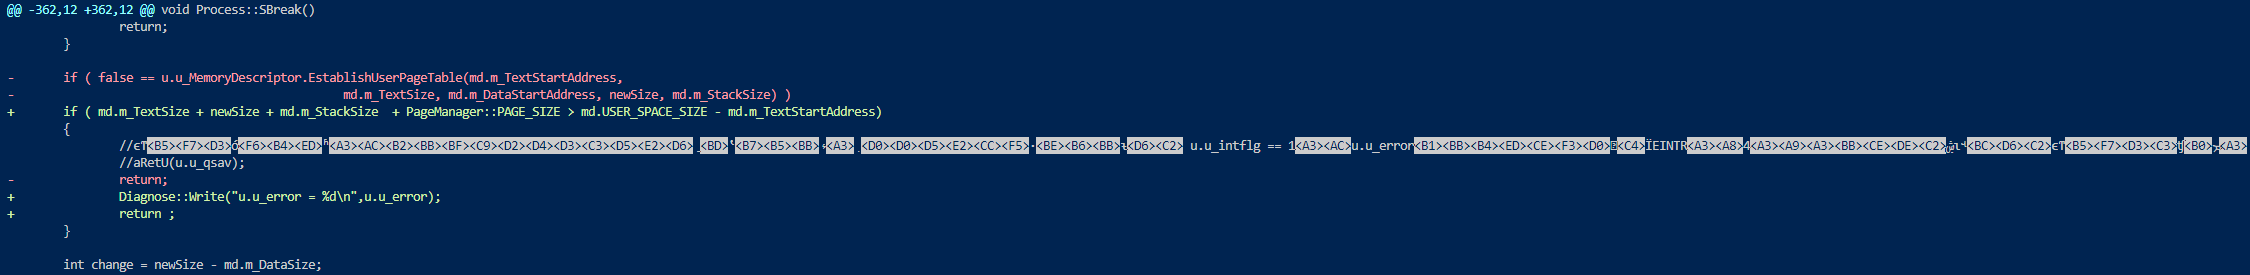
\includegraphics[width=\textwidth]{images/SBreak.png}
    \caption{调整 \texttt{SBreak}对 \texttt{EstablishUserPageTable}的调用}\label{SBtack}
\end{figure}

\begin{figure}[!htbp]
    \centering
    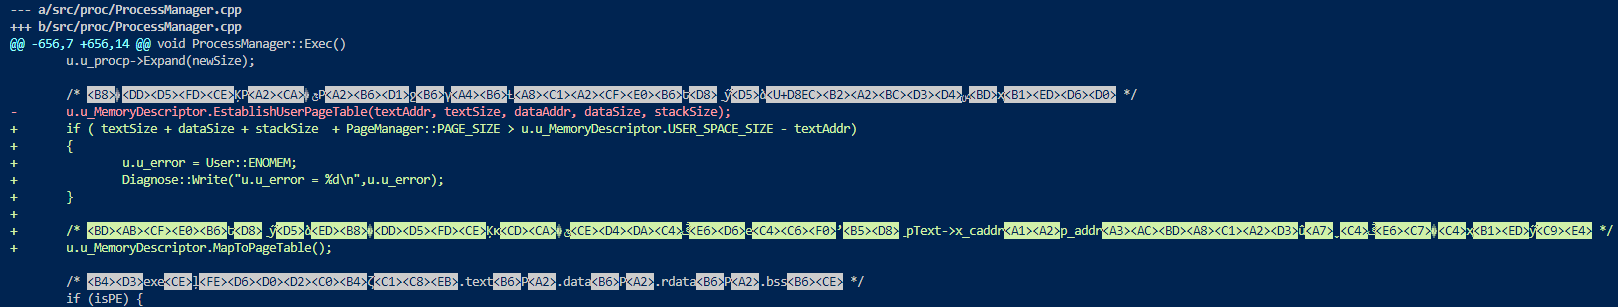
\includegraphics[width=\textwidth]{images/Exec.png}
    \caption{调整 \texttt{Exec}对 \texttt{EstablishUserPageTable}的调用}\label{Exec}
\end{figure}

\clearpage
\subsection{调试验证新的页表系统}

  如图\ref{3}所示, \texttt{showStack}运行结果正确。

\begin{figure}[!htbp]
    \centering
    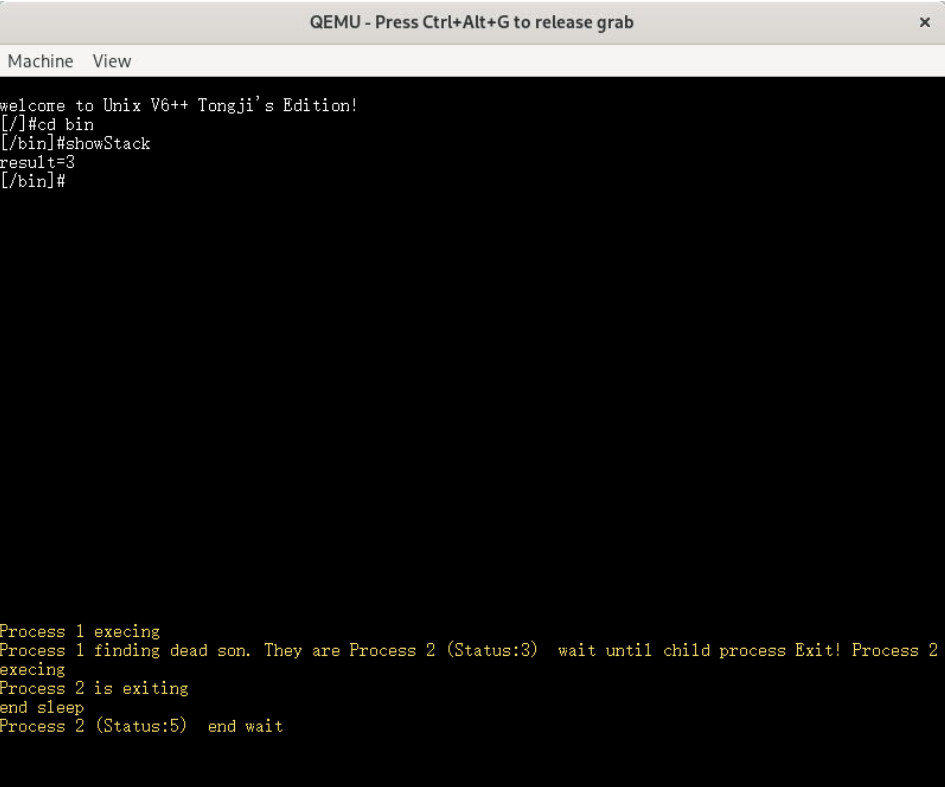
\includegraphics[width=\textwidth]{images/3.png}
    \caption{\texttt{showStack}的运行结果}\label{3}
\end{figure}

  如表\ref{MemoryDescriptorBefore},\ref{MemoryDescriptorAfter}所示, \texttt{MemoryDescriptor}类的成员变量在修改前后的唯一区别在于 相对地址映射表起始逻辑地址\texttt{m\_UserPageTableArray}变为了
用户态页表起始逻辑地址\texttt{UserPageTableArray}。

\begin{table}[!p]
    \centering
 \begin{tabular}{lll}\toprule
    变量名称      &含义         &值        \\\midrule
   \textit{USER\_SPACE\_SIZE }&用户态空间大小            &0x0080 0000=8M               \\
   \textit{USER\_SPACE\_PAGE\_TABLE\_CNT     }&用户态页表数量            &2                            \\
   \textit{USER\_SPACE\_START\_ADDRESS       }&用户态空间起始逻辑地址        &0                            \\
   \textit{m\_UserPageTableArray             }&相对地址映射表起始逻辑地址      &0xC020 8000=3G+2M+32K                  \\
   \textit{m\_TextStartAddress               }&代码段起始逻辑地址      &0x0040 1000=4M+4K                      \\
   \textit{m\_TextSize                       }&代码段大小          &0x3000=12K                      \\
   \textit{m\_DataStartAddress               }&数据段起始逻辑地址      &0x0040 4000=4M+16K                      \\
   \textit{m\_DataSize                       }&数据段大小          &0x5000=20K                      \\
   \textit{m\_StackSize                       }&堆栈段大小          &0x1000=4K                      \\
   \bottomrule
\end{tabular}
\caption{修改前的MemoryDecriptor结构}\label{MemoryDescriptorBefore}
\end{table}

\begin{table}[!h]
    \centering
 \begin{tabular}{lll}\toprule
    变量名称      &含义         &值        \\\midrule
   \textit{USER\_SPACE\_SIZE }&用户态空间大小            &0x0080 0000=8M               \\
   \textit{USER\_SPACE\_PAGE\_TABLE\_CNT     }&用户态页表数量            &2                            \\
   \textit{USER\_SPACE\_START\_ADDRESS       }&用户态空间起始逻辑地址        &0                            \\
   \textit{m\_TextStartAddress               }&代码段起始逻辑地址      &0x0040 1000=4M+4K                      \\
   \textit{m\_TextSize                       }&代码段大小          &0x3000=12K                      \\
   \textit{m\_DataStartAddress               }&数据段起始逻辑地址      &0x0040 4000=4M+16K                      \\
   \textit{m\_DataSize                       }&数据段大小          &0x5000=20K                      \\
   \textit{m\_StackSize                       }&堆栈段大小          &0x1000=4K                      \\
   \textit{UserPageTableArray             }&用户态页表起始逻辑地址      &0xC020 0000=3G+2M                  \\
   \bottomrule
\end{tabular}
\caption{修改后的MemoryDecriptor结构}\label{MemoryDescriptorAfter}
\end{table}

  如图\ref{relative_mem}所示,实验三中相对虚实地址映射表所在内存单元现在的显示的内容为全1。

\begin{Verbatim}[frame=single,fontsize=\small]
    -exec x /20xw 0xC0209004
    0xc0209004:	0xffffffff	0xffffffff	0xffffffff	0xffffffff
    0xc0209014:	0xffffffff	0xffffffff	0xffffffff	0xffffffff
    0xc0209024:	0xffffffff	0xffffffff	0xffffffff	0xffffffff
    0xc0209034:	0xffffffff	0xffffffff	0xffffffff	0xffffffff
    0xc0209044:	0xffffffff	0xffffffff	0xffffffff	0xffffffff
    -exec x /4xw 0xC0209FF0
    0xc0209ff0:	0xffffffff	0xffffffff	0xffffffff	0xffffffff
\end{Verbatim}
\captionof{figure}{视察相对虚实地址映射表所在内存空间}\label{relative_mem}

  逻辑地址3G+2M-3G+2M+4K-1内装有一级页表。

\begin{Verbatim}[frame=single,fontsize=\small]
    -exec x/4xw 0xC0200000
    0xc0200000:	0x00202027	0x00203027	0x00000000	0x00000000
    -exec x/4xw 0xC0200C00
    0xc0200c00:	0x00201023	0x00000000	0x00000000	0x00000000
\end{Verbatim}
\captionof{figure}{视察一级页表所在内存空间}\label{relative_directory}

  逻辑地址3G+2M+4K-3G+2M+8K-1内装有第768张二级页表。

\begin{Verbatim}[frame=single,fontsize=\small]
    -exec x/4xw 0xC0201000
    0xc0201000:	0x00000003	0x00001003	0x00002003	0x00003003
    -exec x/4xw 0xC0201FF0
    0xc0201ff0:	0x003fc003	0x003fd003	0x003fe003	0x00411063
\end{Verbatim}
\captionof{figure}{视察第768张二级页表所在内存空间}\label{mem768}

  逻辑地址3G+2M+8K-3G+2M+12K-1内装有第0张二级页表。

\begin{Verbatim}[frame=single,fontsize=\small]
    -exec x/20xw 0xC0202000
    0xc0202000:	0x00000067	0x00001004	0x00002004	0x00003004
    0xc0202010:	0x00004006	0x00005006	0x00006026	0x00007006
    0xc0202020:	0x00008006	0x00009006	0x0000a006	0x0000b006
    0xc0202030:	0x0000c006	0x0000d006	0x0000e006	0x0000f006
    0xc0202040:	0x00010006	0x00011006	0x00012006	0x00013006
\end{Verbatim}
\captionof{figure}{视察第0张二级页表所在内存空间}\label{mem0}

  逻辑地址3G+2M+12K-3G+2M+16K-1内装有第1张二级页表。

\begin{Verbatim}[frame=single,fontsize=\small]
    -exec x/12xw 0xC0203000
    0xc0203000:	0x00400006	0x0040e065	0x0040f065	0x00410065
    0xc0203010:	0x00412067	0x00413067	0x00414067	0x00415067
    0xc0203020:	0x00416067	0x00412066	0x00413066	0x0040b006
    -exec x/4xw 0xC0203FF0
    0xc0203ff0:	0x007fc006	0x007fd006	0x007fe006	0x00417067
\end{Verbatim}
\captionof{figure}{视察第1张二级页表所在内存空间}\label{mem1}

  经过对比,代码段、数据段、堆栈段和PPDA区对应页框的物理页框号与实验三中观察得到的一致,其余物理页框略有出入。

  上述内容说明再移除相对虚实地址映射表后,新的页表系统工作正常。
\clearpage